\documentclass[fleqn]{article}

\usepackage{polski}
\usepackage[utf8]{inputenc}
\usepackage[polish]{babel}
\usepackage{parskip}
\usepackage{icomma}
\usepackage[a4paper,includeheadfoot,margin=1.27cm]{geometry}
\usepackage{float}
\usepackage{graphicx}
\usepackage{amsmath}
\usepackage[hypcap=true]{subcaption}
\usepackage{xcolor}
\usepackage{transparent}
\usepackage{listings}
\usepackage[colorlinks=true, linkcolor=blue, pdfborder={0 0 0}]{hyperref}

\renewcommand\thesection{\arabic{section}.}
\renewcommand\thesubsection{\alph{subsection})}
\renewcommand\thesubsubsection{}
\newcommand\square[1]{
	\fcolorbox{black}{#1}{\rule{0pt}{6pt}\rule{6pt}{0pt}}
}

\brokenpenalty=1000
\clubpenalty=1000
\widowpenalty=1000

\title{TM -- Laboratorium 3. \\ \large Licznik 8-bitowy – zerowanie, zliczanie w górę do zadanej wartości – kod NKB}
\author{Krystian Chachuła \\ Dawid Gruszczyński \\ Marcin Skrzypkowski}

\begin{document}

\maketitle

\setcounter{page}{0}
\thispagestyle{empty}

\pagebreak

\setcounter{page}{1}

\section{Wstęp}

Na trzecim laboratorium mieliśmy za zadanie, korzystając z modułu mikrokontrolera MSP430 oraz innych modułów SML-3, zaprojektować i zrealizować licznik zliczający w górę w kodzie NKB z możliwością asynchronicznego zerowania jego zawartości.
Sterowanie licznikiem miało odbywać się za pomocą dwóch przycisków (CLK aktywne zboczem oraz CLR aktywne poziomem).
Dodatkowym wymogiem zadania była realizacja programowej eliminacji drgań styków oraz obsługa przynajmniej jednego z przycisków z użyciem przerwań.

Zaprojektowany przed laboratorium układ zbudowaliśmy z następujących układów SML-3:

\begin{itemize}
	\item \textbf{10\_PS1} (moduł zasilacza)
	\item \textbf{160\_7SEG2} (moduł wyświetlacza 7 segmentowego)
	\item \textbf{120\_IN8} (zestaw 8 monostabilnych wyłączników)
	\item \textbf{451\_IN\_4xHEX} (moduł przełączników szesnastkowych)
	\item \textbf{570\_MSP430F14x} (moduł mikrokontrolera Texas Instruments serii MSP430f14x lub F16x)
\end{itemize}

\section{Implementacja licznika}

Projektowanie rozpoczęliśmy od stworzenia grafu stanów, który przedstawiał ogólny schemat działania licznika.
%TODO ogarnąć grafuu

\begin{figure}[H]
	\centering
	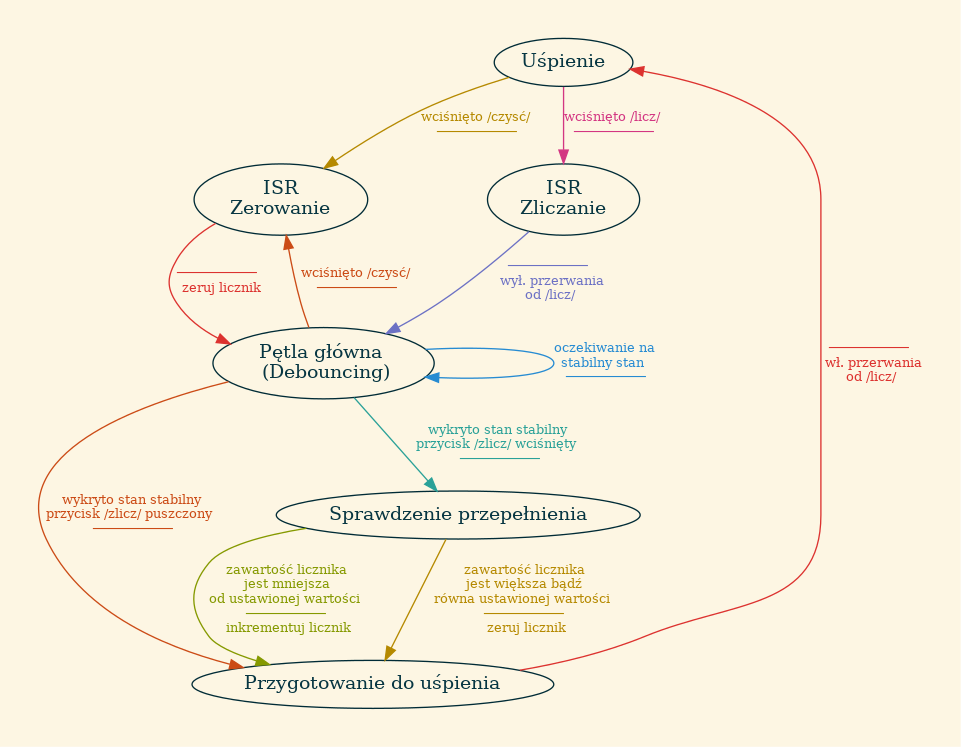
\includegraphics[width=\textwidth]{assets/graph.png}
	\caption{Graf automatu stanów}
	\label{fig:graph}
\end{figure}


Na początku pracy, mikrokontroler znajduje się w stanie uśpienia. Wybudzenie następuje tylko w przypadku wystąpienia przerwania z portu P1 (zbocze przycisku CLK) lub portu P2 (zbocze przycisku CLR). Następnie następuje przejście do obsługi zgłoszonego przerwania. W przypadku przerwania od przycisku CLK, wyłączane są tylko przerwania generowane przez ten przycisk oraz trwale wybudzany jest mikrokontroler (przejście do pętli głównej programu). W przypadku perwania od przycisku CLR zerowane jest wyjście licznika, zerowana jest zawartość rejestru służącego do usuwania drgań styków (rejest R5) oraz wyłączane są przerwania od przycisku CLK (na czas trzymania wciśniętego przycisku CLR nie chcemy by istaniała możliwość wywołania przerwania zliczającego). Wybudzany jest także trwale mikrokontroler. Przerwania zliczające mogą być wywoływane tylko w momencie gdy mikrokontroler jest w stanie uśpienia, natomiast przerwania zerujące mogą być wywoływane w każdym miejscu poza sekcją krytyczną związaną z inkrementacją licznika. Przerwania nie mogą być zagnieżdżane. W pętli głównej programu, sprawdzane jest czy wciśnięty jest przycisk zerujący (w przypadku zerowania licznika blokujemy możliwośc inkrementacji do momentu puszczeniu przycisku CLR) oraz czy wciśnięty jest przycisk zliczania (eliminacja drgań w przypadku inkrementacji licznika). Eliminacja drgań odbywa się poprzez zliczanie do pewnej wartości za pomocą rejestru R5. Po pomyślnym przeczekaniu drgań następuje inkrementacja licznika. Proces eliminacji drgań może zostać przerwany przez wciśnięcie przycisku CLR, w takim przypadku licznik jest zerowany a proces inkrementacji zostaje przerwany. Po zakończeniu zerowania lub inkremetacji licznika, zerowany jest rejestr R5 oraz włączane są przerwania przycisku zliczającego, następnie mikrokontroler ponownie jest usypiany.

Na podstawie grafu powstał kod napisany w języku Assembly.

\pagebreak

\section{Program}
%TODO Opis kodu

%TODO kod
\lstinputlisting[lastline=55]{src/main.asm}

\pagebreak

\lstinputlisting[firstline=56]{src/main.asm}

\pagebreak

\section{Podłączenie procesora}

%\begin{figure}[H]
	%\centering
	%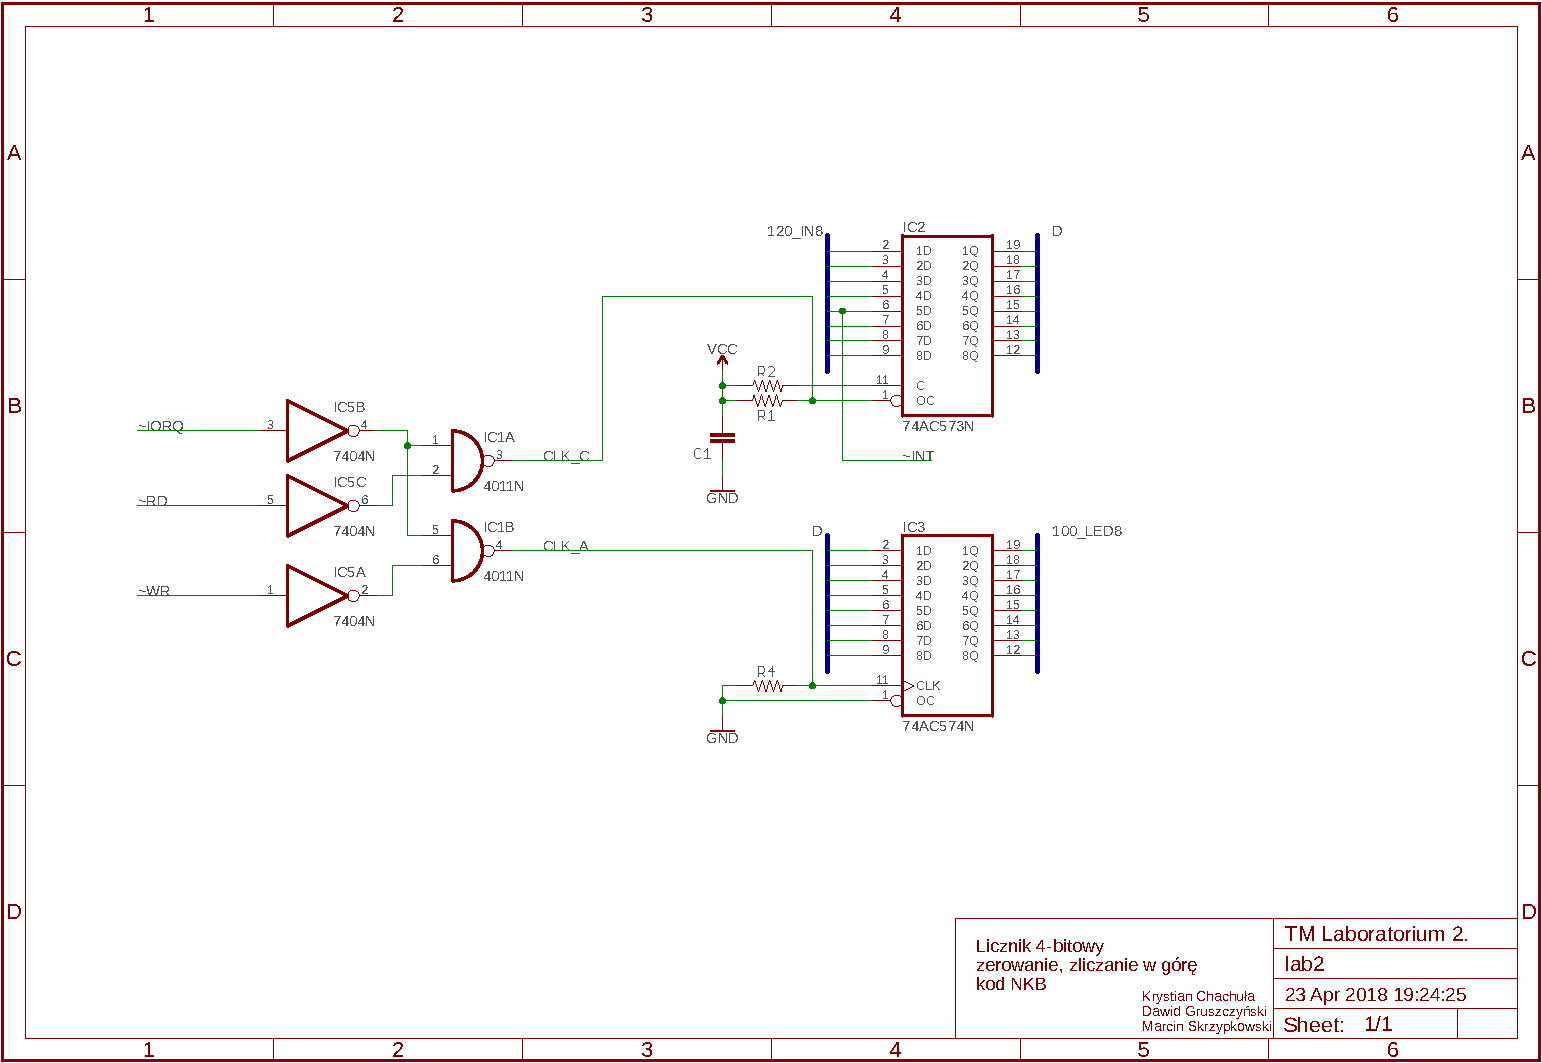
\includegraphics[width=\textwidth]{img/schematic.pdf}
	%\caption{Schemat układu}
	%\label{fig:schematic}
%\end{figure}

Przyciski sterujące pracą licznika podłaczyliśmy do portów P1 oraz P2, (przycisk CLR do pinu 1 portu P1, ponieważ musi on posiadać większy priorytet, natomiast przycisk CLK do pinu 4 portu P2). Wyjściem licznika jest port P3 skonfigurowany jako wyjście, którego zawartość wyświetlana jest za pomocą modułu wyświetlacza 7 segmentowego. Do wczytywania wartości zadanej, do której ma zliczać licznik, wykorzystaliśmy port P4 skonfigurowany jako wejście. Jest on bezpośrednio podłaczony do modułu przełączników szesnatkowych.

\section{Możliwości rozwoju}

Możliwym udoskonaleniem zadania byłoby dodatkowe sprawdzanie poprawności odczytu wartości zadanej z modułu przełączników szesnastkowych. Odczyt w złym momencie może powodować przekłamania niektórych bitów spowodowane przełączaniem między pozycjami. Aby mieć pewność, że odczytany stan jest stabilny należy kilkukrotnie odczytać sygnał wejściowy na porcie P4 i sprawdzić czy odczytane wartości nie rożnią się między sobą. W przypadku różnic należy przeprowadzać ponowne odczyty aż do uzyskania wartości stabilnej.

\end{document}
\grid
